% Chapter Template
\chapter{Project Overview5-10p} % Main chapter title

\label{Chapter2} % For referencing the chapter elsewhere, use \ref{Chapter1} 

%----------------------------------------------------------------------------------------
%	SECTION 1
%----------------------------------------------------------------------------------------
Refering to \ref{fig:gartnerIoT}, we analyzed the existing architecture of the escape room.
\begin{description}
	\item[Device Layer]\hfill \\
	      The Device Layer consisted of different Arduinos as Actuators, and riddle-depending sensors for each riddle.
	      The Gateway device was an Adafruit Feather 32u4.
	\item[Communication Layer]\hfill \\
	      The Communication within the room was set-up with RFM69HCW Transceiver modules.\parencite{radiorange}
	      The RFM69HCW is very cheap and easy to use and setup Transceiver. They do packetization, error correction and auto-retransmit which makes them easier to handle than other communication systems.
	      They are designed for point-to-multipoint communication with one Transceiver set-up as a Gateway node which sends data to the other Transceivers in the room.
	      There are two open-source libaries for the RFM69HCW, the LowPowerlab \parencite{LowPowerlab} and Radiohead \parencite{Radiohead} libary.
	      The escape room used the LowPowerlab libary since the architect was familiar with the libary.
          Now-a-days the Radiohead libary is the recommended libary since it's documented more thorough and kept up-to-date.
          The Gateway Transceiver is connected to a PC through the Serial Port. Any node is recognized by a different nodeID and the Gateway with a specified GatewayID. For security-reasons, password-encryption is used between the nodes. 
          From there, a C++-Server would forward those messages to any Tcp-Client listening.    
          The Server would forward any messages coming from the TCP-Client back to the Serialport just as well.
	\item[Information Layer]\hfill \\
        The Information Layer was build around a simple Event Model: the Transceivers would send codes in a "Number/Number/Number..."-structure. 
        A node could be identified through the string it sent, since the first number would be the node's adressing number. 
        The other numbers would represent the current state of the Arduino with a "Switch-Case" Szenario \ref{fig:switchCase}. 
	\item[Function Layer]\hfill \\
        If the Code matched with the Tcp-Clients list (in our case, in a Unity application), a Video in Unity would be played and Unity would send a "reset" code to the matching riddle. 
        Both lists were defined statically.
	\item[Process Layer]\hfill \\
	Apart form the main functionality, offered the C++-Server a communication window where Serialport-messages 
    could be seen and sent manually. \ref{fig:c++window}.

\end{description}
\ref{fig:oldEscapeUml} provides further insight into the architecture
\begin{figure}[th]
	\centering
	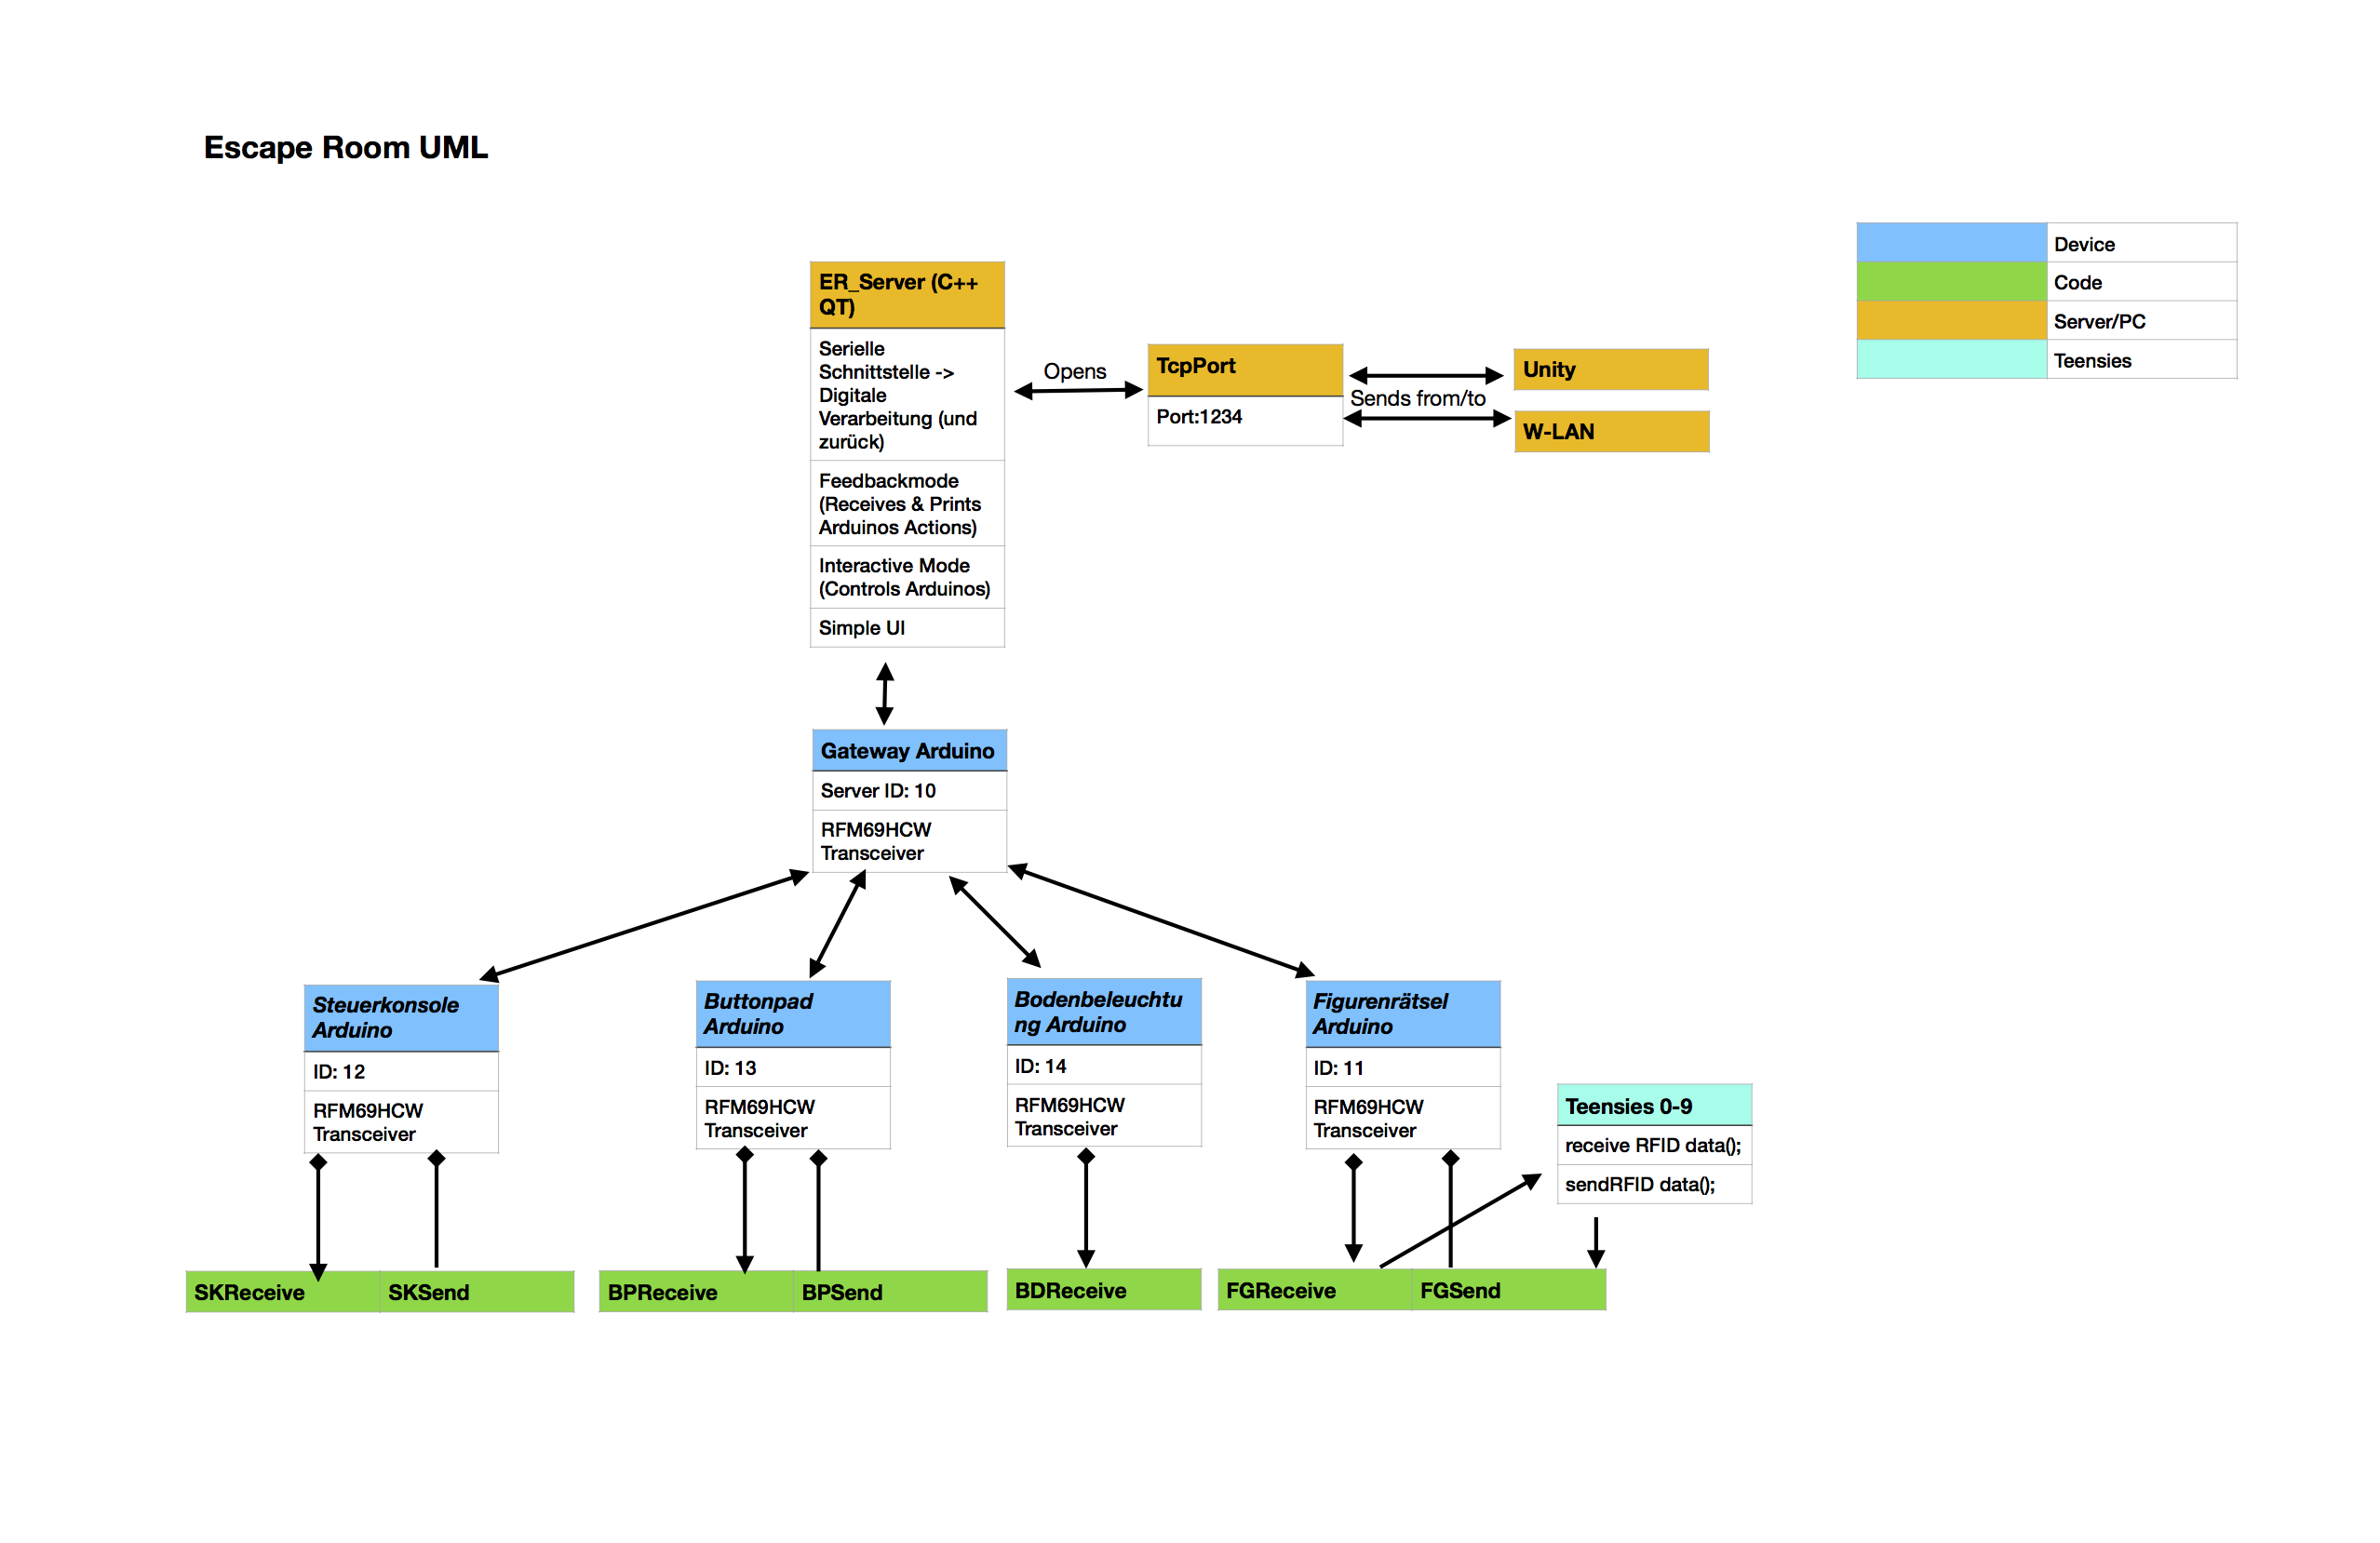
\includegraphics[width=75mm,scale=0.75]{Figures/oldEscapeUml}
	\decoRule
	\caption[UML]{The old escape room structure.}
	\label{fig:oldEscapeUml}
\end{figure}
\begin{figure}[th]
    %\includegraphics[width=75mm,scale=0.75]{Figures/switchCase}
    \decoRule
    \caption[messages]{Example of the messages defined in the Arduino}
    \label{fig:switchCase}
\end{figure}
\begin{figure}[th]
    %\includegraphics[width=75mm,scale=0.75]{Figures/c++window}
    \decoRule
    \caption[messages]{Example of the messages defined in the Arduino}
    \label{fig:c++window}
\end{figure}

%SECTION TWOOO
\subsection{Analysis}
In 2009, Kim Goodwin stated that 
„Interactive products and services tend to require four different types of work from users: 
cognitive, visual, memory, and physical“ \parencite{designDigitalAge} 
While an IoT-System is not always interactive, our goal was very interaction-orientated: We wanted to help engineers expand the existing room which would require 
interaction with the Device-Layer (if they wanted to add hardware-functionality) 
and the Process-Layer (if they wanted to add software-functionality).
Therefore it makes sense to analyze our specific project with those aspects in mind. 
The room was well designed for the user, and the four areas of cognitive, visual, memory and physical work involved for an escape room customer would already be pretty low.

\subsubsection{Cognitive Work}
Engineering products usually demands some kind of cognitive work. Still, there are hurdles that can be avoided,
like finding out wether to click "yes" "no" or "cancel" in a confirmation dialog can be made clearer if the question is phrased easily.
In our case, the Cognitive Work needed to add a riddle or a functionality is enormous:
Device Layer:
\begin{enumerate}
    \item The user needs to understand the transport protocol and therefore needs to 
    \begin{enumerate}
        \item Set-Up the RFM69HCW with an Arduino or an Adafruit Feather, which requires drivers and another libary
        \item understand the communication within the LowPowerlab-libary
        \item look up the other riddles codes to avoid using a %belegte nodeID
    \end{enumerate}   
    \item understand Arduino-coding 
    \item understand working with the "Switch-Case"-scenario used for communication 
\end{enumerate}  
Process Layer:
\begin{enumerate}
    \item understand C++ to change the Server (f.e. to communicate with an upper-level protocol)
    \item understand C\# and Low-Level-Socket communication to make changes in Unity 
    and get an Overview about the communication since it's in separate files (one File per Video and one for the Tcp Socket) 
\end{enumerate}  

\subsubsection{Visual Work}
Visual work means how much the user has to search for the answers in a project visually.
The given interface was clear, but lacked in buttons for often used functionalities (reset, "send feedback"...).

\subsubsection{Memory Work}
Memory work is measured in how much a user has to remember to succeed in a task. 
Typical examples are passwords, command names, and file names.
In our current state, the architecture demands a lot of memory work from a developer:
\begin{enumerate}
    \item the developer has to translate "Number/Number/Number..." codes whenever he wants to understand the serialport-messages 
    \item the developer has to remember a different code when he wants to send an order to the device
    \item anyone who starts the room has to remember to first start the c++ server and afterwards the unity application on the desktop, or connection will fail.
    \item the developer has to enable the "enable feedback" mode for each node manually if he wants to see all messages send
    \item the developer has to enable another mode if he wants to interact with the riddles, and the riddle won't react hardware-wise in that mode.
\end{enumerate} 

\subsubsection{Physical Work}
IoT-Projects always involve some kind of physical work for a developer: you have to switch between hardware and software to test the devices for example.
The escape room fits into that scenario but doesn't make testing physically harder than it needs to be in most aspects. 
One aspect that makes changes harder is seemingly unavoidable - most of the hardware is hidden, therefore mostly difficult to access. 
Since an escape room is made for customers who expect the illusion of in this case, a spaceship, 
it wouldn't fit to have hardware with "do not touch" signs all over the place lying around.

\subsubsection{Consequences}
//da fehlt noch viel

This analysis showed the projects strengths and weaknesses. The next step was to estimate the workload and possibilities 
we had with our limited resources to change the project for the better. 
As mentioned earlier, IoT-Projects typically follow a SoA %Reference to abkürzung!
to keep the project flexible and expandable. 
%ergänzen!

\begin{figure}[th]
    \centering
    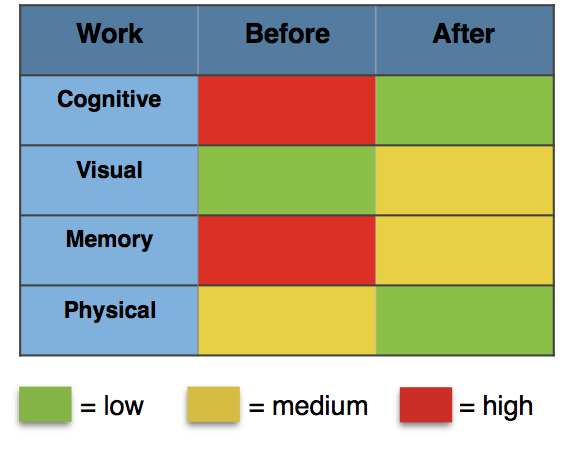
\includegraphics[width=50mm,scale=.5]{Figures/workload}
    \decoRule
    \caption[workload]{Workload of the different aspects color-coded}
    \label{fig:workload}
\end{figure}
